\subsection{Sequential Monte Carlo}
In this case, we follow the Algorithm~\ref{alg:sampling/part-fil/part-fil}. We show in Figure~\ref{fig:pprog/how/figures/smc} an illustration for one SMC iteration, adopting the notation in this chapter.
\begin{figure}[!htb]
\centering
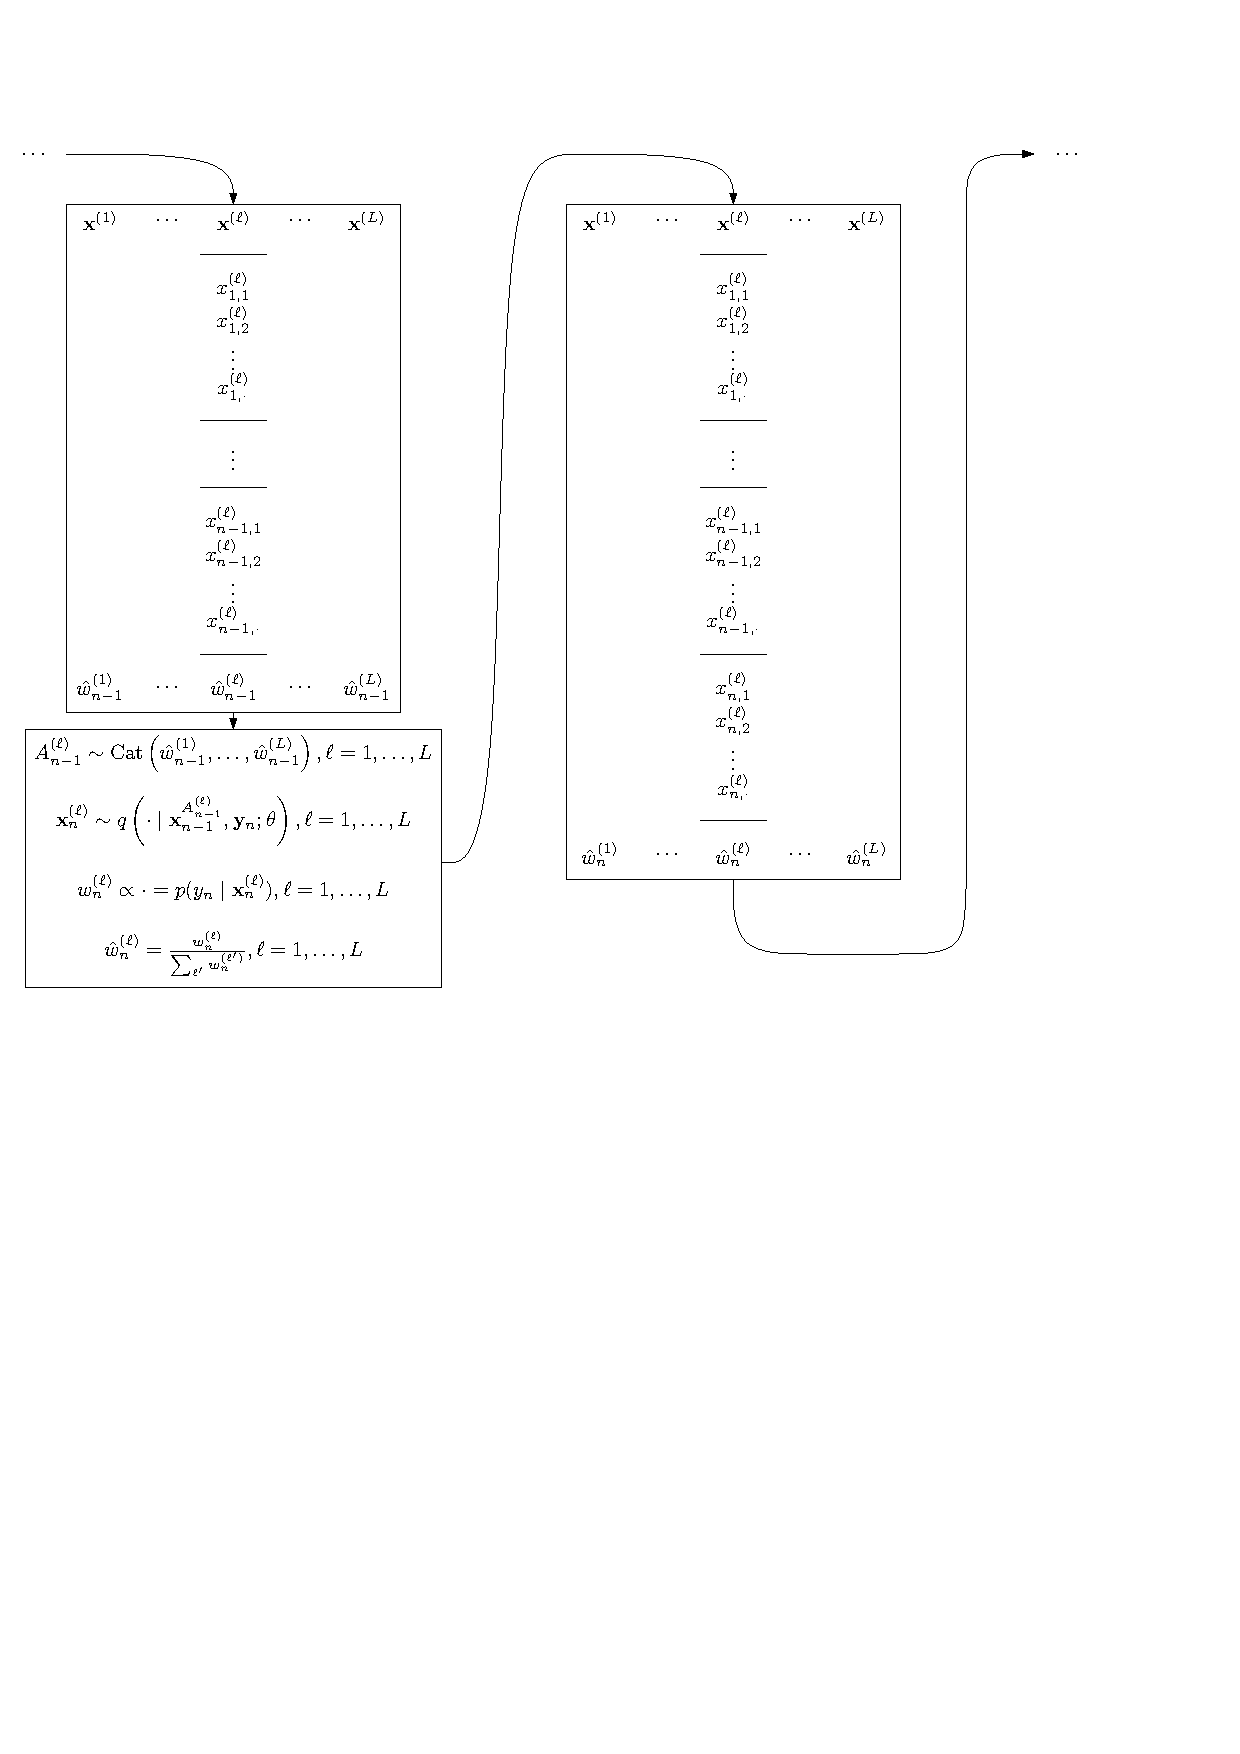
\includegraphics[scale=0.75]{pprog/how/figures/smc/smc}
\caption{Illustration of the SMC iteration $n$.}
\label{fig:pprog/how/figures/smc}
\end{figure}

\begin{itemize}
	\item The proposal is done by just continuing interpretation, i.e. $q\left(\vec x_n^{(\ell)} \mid \vec x_{n - 1}^{A_{n - 1}^{(\ell)}}, \vec y_n; \vec \theta\right) = p\left(\vec x_n^{(\ell)} \mid \vec x_{n - 1}^{A_{n - 1}^{(\ell)}} \right)$.
	\item The weights calculation then simplifies to $p\left(y_n \mid \vec x_{n - 1}^{A_{n - 1}^{(\ell)}}\right)$. TODO: Verify.
	\item Whenever a \verb!predict! is needed, we can resample from
		\begin{equation*}
			\hat p(\mathrm d \vec x_{1:n} \mid y_{1:n}; \vec \theta) = \sum_\ell \hat w_t^{(\ell)} \delta_{\vec x_{1:n}^{(\ell)}}(\mathrm d \vec x_{1:n})
		\end{equation*}
		to get a sample from the posterior.
\end{itemize}